\documentclass[letterpaper]{article}
\title{CSE 546 Machine Learning, Autumn 2013 \\ Homework 3}
\date{Shrainik Jain, 1323338}
\usepackage{hyperref}

\usepackage[margin=1.5in]{geometry}

\usepackage{amsmath,amsfonts}
\usepackage{capt-of}
\usepackage{url}
\usepackage{graphicx}
\usepackage{color}
\usepackage{bbm}
\usepackage{enumerate}
\newcommand{\carlos}[1]{\textcolor{red}{Carlos: #1}}
\newcommand{\field}[1]{\mathbb{#1}} 
\newcommand{\hide}[1]{#1}
\newcommand{\pd}[2]{\frac{\partial #1}{\partial #2}}
\providecommand{\m}[1]{\mathbf{#1}}
\providecommand{\norm}[1]{\left\|#1\right\|}
\providecommand{\sign}[1]{\text{sign}\left(#1\right)}
\DeclareMathOperator*{\argmin}{arg\,min}
\providecommand{\what}{\m{\hat{w}}}

\begin{document}

\maketitle


\section{Fitting an SVM classifier by hand [25 Points]}
\begin{enumerate}
\item $\phi(x) = [1, \sqrt{2}x,x^2]^T$. This gives $\phi(data) = [1, \sqrt{2}*0, 0^2]^T , [1, \sqrt{2}*\sqrt{2}, \sqrt{2}^2]^T = [1, 0, 0]^T, [1, 2, 2]^T$. The following figures show the decision boundaries and margin which will be used as a reference for this problem.\\
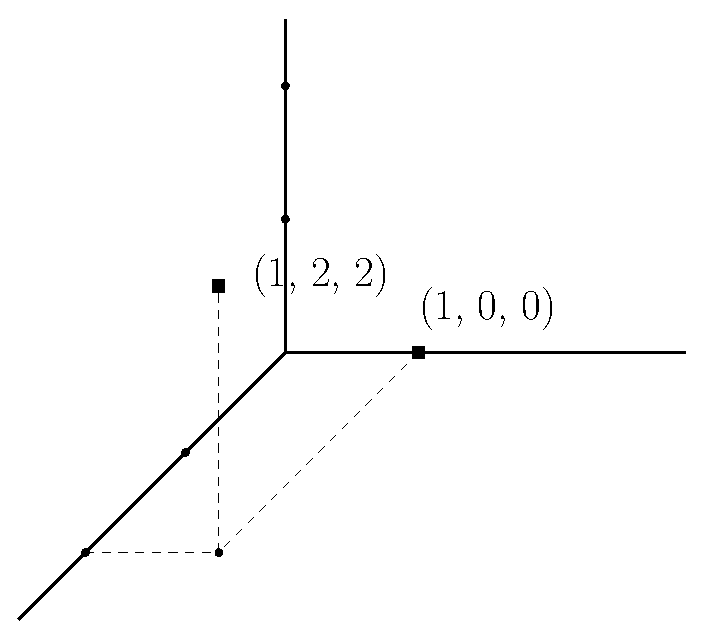
\includegraphics[width = 2.5in,keepaspectratio]{HW3_figure1.eps}
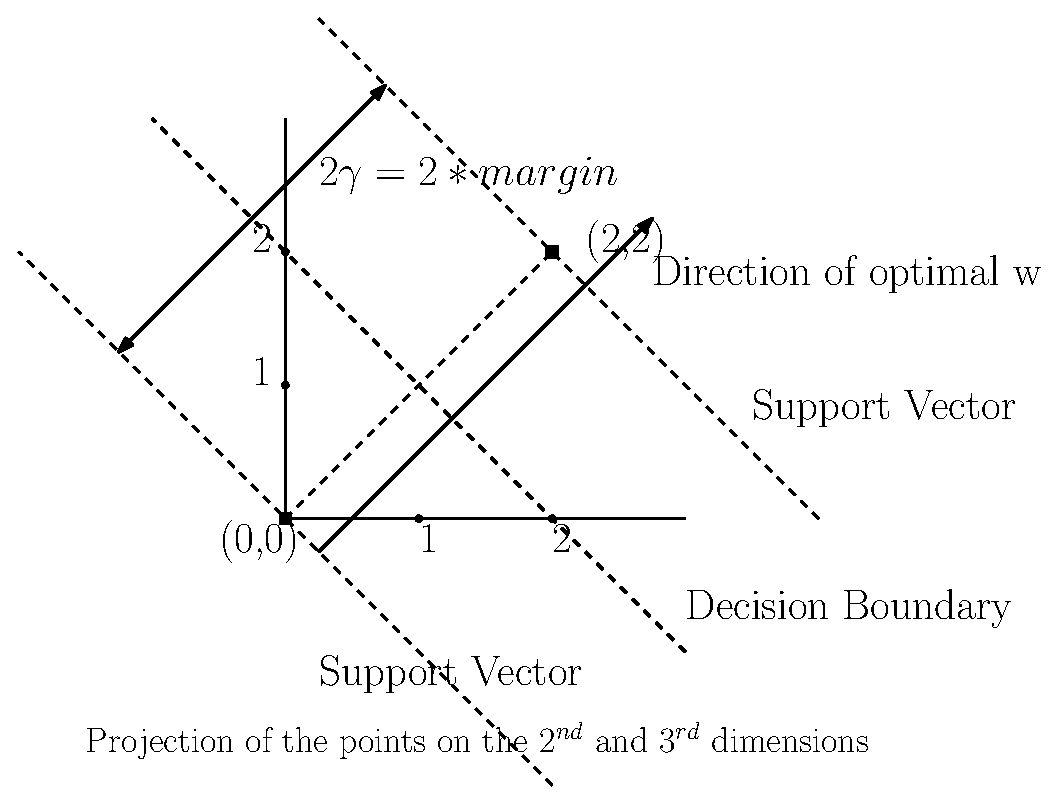
\includegraphics[width = 3in, keepaspectratio]{HW3_figure2.eps}

From the figures it is clear that optimal w is parallel to the line joining the points $[1, 0, 0]^T  \&  [1, 2, 2]^T$. One such
\begin{equation}
 w = [0, 2, 2] \,\,\, ...(Ans)
\end{equation}

\item As shown in the second figure the margin is half of the distance between the points $[1, 0, 0]^T  \&  [1, 2, 2]^T$.
\begin{equation}
\gamma = \frac{1}{2}\sqrt{(1-1)^2 + (2-0) + (2-0)^2} = \sqrt{2} \,\,\, ...(Ans)
\end{equation}

\item 
Let the optimal $w = [w_1, w_2, w_3]$
\begin{equation}
\gamma = \frac{1}{||w||} \Rightarrow ||w|| = \frac{1}{\sqrt{2}} \Rightarrow (w_1^2 + w_2^2 + w_3^2) = \frac{1}{2}
\end{equation}

From figures we see that w is parallel to [0, 2, 2] and passes through origin. Hence,
\begin{equation}
w_1 = 0 \,\, \& \,\,w_2 = w_3
\end{equation}

Plugging into the previous equation we get:
\begin{equation}
2w_2^2 = \frac{1}{2} \Rightarrow  [w_1, w_2, w_3] = [0, \frac{1}{2}, \frac{1}{2}] \,\,\, ...(Ans)
\end{equation}

\item We have:
\begin{equation}
y_1(w^T \phi(x_1) + w_0) \geq 1
\label{eq:condit1}
\end{equation}
\vspace{-1cm}

\begin{equation}
y_2(w^T \phi(x_2) + w_0) \geq 1
\label{eq:condit2}
\end{equation}

from these equations and the results from the previous parts, we get:
\begin{equation}
-1(0*1 + 1/2 * 0 + 1/2 * 0 + w_0) \geq 1 \Rightarrow w_0 \leq -1
\end{equation}
and
\begin{equation}
1(0*1 + 1/2 * 2 + 1/2 * 2 + w_0) \geq 1 \Rightarrow w_0 \geq -1
\end{equation}

This implies that  $w_0 = -1$  ... (Ans)

\item Using the results from the previous parts:
\begin{equation}
f(x) = -1 + \frac{x}{\sqrt{2}} + \frac{x^2}{2}
\end{equation}
The plot for the function:\\
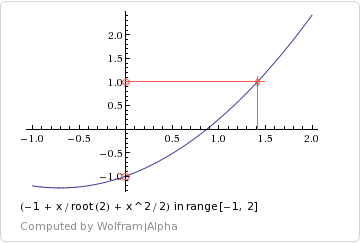
\includegraphics[width = 4in, keepaspectratio]{HW3_q1plot.png}
\end{enumerate}

\section{Manual calculation of one round of EM for a GMM [30 points]}
\subsection*{M step}
\begin{enumerate}
\item The log likelihood function we are trying to optimize is:
\begin{equation}
Q(\theta, \theta^{(t-1)}) = \sum_{i}{\sum_{k}{r_{ic}log(\pi_{c})}}  + \sum_{i}{\sum_{k}{r_{ic}log(p(x_i|\theta_c))}} \,\,\, ...(Ans)
\end{equation}
taken from Murphy, page 351.
\item
We know that:
\begin{equation}
\pi_c = \frac{1}{N}\sum_i{r_{ic}} = \frac{r_c}{N}
\end{equation}
Hence,
\begin{equation}
\pi_1 = \frac{1}{3}(1+0.4+0) = \frac{1.4}{3} = \frac{7}{15} \,\,\, ...(Ans)
\end{equation}
\begin{equation}
\pi_2 = \frac{1}{3}(0+0.6+1) = \frac{1.6}{3} = \frac{8}{15} \,\,\, ...(Ans)
\end{equation}
\item
We have: 
\begin{equation}
\mu_c = \frac{\sum_i{r_{ic}x_i}}{r_c}
\end{equation}
Plugging in the values we get:
\begin{equation}
\mu_1 = \frac{1*1 + 0.4*10 + 0*20}{1 + 0.4 + 0} = \frac{5}{1.4} = \frac{25}{7} \,\,\,...(Ans)
\end{equation}
\begin{equation}
\mu_2 = \frac{0*1 + 0.6*10 + 1*20}{1 + 0.6 + 0} = \frac{26}{1.6} = \frac{65}{4} \,\,\,...(Ans)
\end{equation}
\item
We have,
\begin{equation}
\Sigma_c = \frac{\sum_i{(r_{ic})(x_i-\mu_c)(x_i - \mu_c)^T}}{r_c}
\end{equation}
and
\begin{equation}
\sigma_c = \sqrt{\Sigma_c}
\end{equation}
Plugging in the values:
\begin{equation}
\Sigma_1 = \frac{1(1-\frac{25}{7})^2 + 0.4(10-\frac{25}{7})^2 + 0(20-\frac{25}{7})^2}{1 + 0.4 + 0} = 16.53 \Rightarrow \sigma_1 = 4.065\,\,\,...(Ans)
\end{equation}

\begin{equation}
\Sigma_2 = \frac{0(1-\frac{65}{4})^2+0.6(10-\frac{65}{4})^2+ 1(20-\frac{65}{4})^2}{0 + 0.6 + 1} = 23.4375 \Rightarrow \sigma_2 = 4.84 \,\,\,...(Ans)
\end{equation}

\end{enumerate}
\subsection*{E step}
\begin{enumerate}
\item The probability of observation $x_i$ belonging to cluster c:
\begin{equation}
r_{ic} = \frac{\pi_kp(x_i|\theta_k^{(t-1)})}{\sum_{c'}{\pi_{c'}p(x_i|\theta_{c'}^{(t-1)})}} \,\,\, ...(Ans)
\end{equation}
where probability follows a Gaussian distribution, i.e.:
\begin{equation}
p(x_i|\theta_c^{(t-1)}) = \frac{1}{\sigma_c\sqrt{2\pi}}\exp{-\frac{1}{2}(\frac{x_i - \mu_c}{\sigma_c})^2}
\end{equation}
taken from Murphy, page 351.
\item
Using the two equations above and plugging in the values, we get: \\
$p(x_1|\theta_1) = \frac{1}{4.065\sqrt{2\pi}}\exp{-\frac{1}{2}(\frac{1 - \frac{25}{7}}{4.065})^2} = 0.0803$\\
$p(x_1|\theta_2) = \frac{1}{4.84\sqrt{2\pi}}\exp{-\frac{1}{2}(\frac{1 - \frac{65}{4}}{4.84})^2} = 0.000575$\\
$p(x_2|\theta_1) = \frac{1}{4.065\sqrt{2\pi}}\exp{-\frac{1}{2}(\frac{10 - \frac{25}{7}}{4.065})^2} = 0.028$\\
$p(x_2|\theta_2) = \frac{1}{4.84\sqrt{2\pi}}\exp{-\frac{1}{2}(\frac{10 - \frac{65}{4}}{4.84})^2}$ = 0.0358\\
$p(x_3|\theta_1) = \frac{1}{4.065\sqrt{2\pi}}\exp{-\frac{1}{2}(\frac{20 - \frac{25}{7}}{4.065})^2} = 0.0000278$\\
$p(x_3|\theta_2) = \frac{1}{4.84\sqrt{2\pi}}\exp{-\frac{1}{2}(\frac{20 - \frac{65}{4}}{4.84})^2}$ = 0.061\\

Hence, 
$r_{11} = \frac{\frac{7}{15}0.0803}{\frac{7}{15}0.0803 + \frac{8}{15}0.000575} = 0.992$\\
$r_{12} = 1 - r_{11} = 1 - 0.992  = 0.008$\\
$r_{21} = \frac{\frac{7}{15}0.028}{\frac{7}{15}0.028 + \frac{8}{15}0.0358} = 0.406$\\
$r_{22} = 1 - r_{21} = 1 - 0.406  = 0.594$\\
$r_{31} = \frac{\frac{7}{15}0.0000278}{\frac{7}{15}0.0000278 + \frac{8}{15}0.061} = 0.00039$\\
$r_{32} = 1 - r_{31} = 1 - 0.00039  = 0.99961$\\

\[ R_{new} = \left( \begin{array}{cc}
0.992 & 0.008 \\
0.406 & 0.594 \\
0.00039 & 0.99961 \end{array} \right)\]  \,\,\, ...(Ans)

\end{enumerate}
\section{Programming Question [45 Points]}

\subsection{Dataset}
No question in this part.

\subsection{Perceptron}
\begin{enumerate}

\item
From the lecture on Oct $28^{th}$, slide 7, we know the following:
\begin{equation}
\hat{y} = sign(\phi(x).w^{(t)}) = sign(\sum_{j \in M^{(t)}}{y^{(j)}\phi(x).\phi(x^{(j)})})
\end{equation}
and
\begin{equation}
sign(\sum_{j \in M^{(t)}}{y^{(j)}\phi(x).\phi(x^{(j)})}) = sign(\sum_{j \in M^{(t)}}{y^{(j)}k(x, x^{(j)})})
\end{equation}
hence the prediction rule is:
\begin{equation}
\hat{y} = sign(\sum_{j \in M^{(t)}}{y^{(j)}k(x, x^{(j)})}) \,\,\, ...(Ans)
\end{equation}
 where $M^{(t)}$ = mistakes till iteration t.

\item See attached code.

\item Plot for average loss at every 100 steps:\\ \\
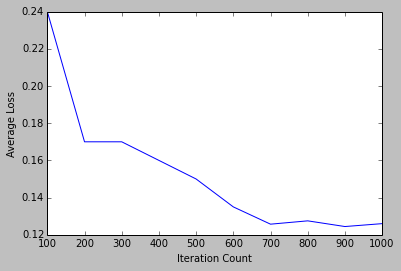
\includegraphics[width = 4.5in,keepaspectratio]{HW3_figure3.png}

\item Plot for the average loss after 1000 iterations for the kernels with increasing degree of polynomials:\\ \\ 
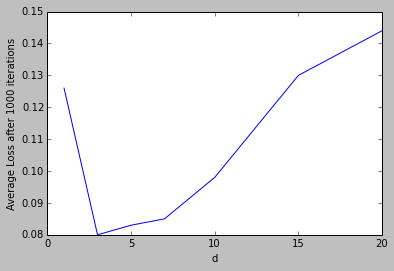
\includegraphics[width = 4.5in, keepaspectratio]{HW3_figure4.png}

\item Plot for average loss at every 100 steps, polynomial kernel with d = 3 vs. gaussian kernel with $\sigma = 1000$:\\  \\
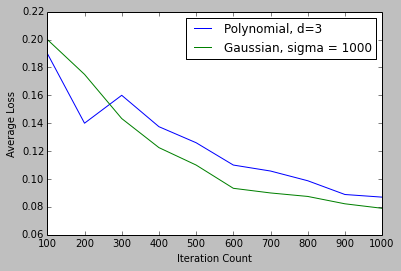
\includegraphics[width = 4.5in, keepaspectratio]{HW3_figure5.png}

\end{enumerate}

\subsection{SVM}
 
\begin{enumerate}

\item Update rules for linear SVM Stochastic gradient descent: 
\begin{equation}
w^{(t+1)} = w^{(t)} + \eta  (C  \mathbb{I}((1-y^{(t)}(w^{(t)}.x^{(t)} + w_0^{(t)}) > 0)) - 2w^{(t)})
\end{equation}

\begin{equation}
w_0^{(t+1)} = w_0^{(t)} + \eta  C  y^{(t)} \,\,\,  ...(Ans)
\end{equation}

\item See attached code.

\item Average loss after every 100 steps for $\eta = 10^{-5}$ and $C = 1$: \\ \\ 
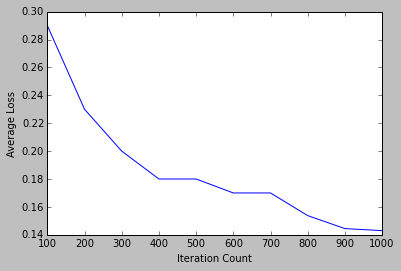
\includegraphics[width = 4.5in, keepaspectratio]{HW3_figure6.png}

\item For SVMs, C is the measure of how much we want to penalize misclassification of data, ie. the categorization error. The objective of SVM is:
\begin{equation}
argmin \,\,\,  ||w||_2^2 + C\sum_{j=1}^N{(1-y^j(w.x^j + w_0))_{+}}
\end{equation}

We started the experiment with C=1 and got some decision rule d1, which misclassified some data points due to linear inseparablity of data. Irrespective of how much we increase C, we will always misclassify these specific linearly inseparable data points (since we are not using features of features). Hence the decision rule doesnt change. It just means that the margin keeps on decreasing.

\item As stated in the previous part, C is the measure of how much we want to penalize misclassification of data. If we increase C, we penalize the mistakes more and decrease the margin. A higher values of C imply that we will get good separation in the data but a smaller margin. Lower values of C imply that we want bigger margins and and care lesser about the number of mistakes in training.\\
The relation with perceptron can be seen as the following:
\begin{itemize}
\item Both SVM and perceptron try to minimize the hinge loss, but SVM has regularization.
\item Lack of regularization in perceptron gives it an exact upper bound on the number of mistakes. In SVM, we can control this upper bound by the regularization constant C. Specifically, lower C $\Rightarrow$ higher bound on number of allowed errors. (which in turn implies we are willing to tolerate errors to get a better separation.)
\end{itemize}

\end{enumerate}

\end{document}